\documentclass[preprint,12pt]{elsarticle}

%% Use the option review to obtain double line spacing
%% \documentclass[preprint,review,12pt]{elsarticle}

%% Use the options 1p,twocolumn; 3p; 3p,twocolumn; 5p; or 5p,twocolumn
%% for a journal layout:
%% \documentclass[final,1p,times]{elsarticle}
%% \documentclass[final,1p,times,twocolumn]{elsarticle}
%% \documentclass[final,3p,times]{elsarticle}
%% \documentclass[final,3p,times,twocolumn]{elsarticle}
%% \documentclass[final,5p,times]{elsarticle}
%% \documentclass[final,5p,times,twocolumn]{elsarticle}

%% The graphicx package provides the includegraphics command.
\usepackage{graphicx}
%% The amssymb package provides various useful mathematical symbols
\usepackage{amssymb}
\usepackage{amsmath}
\usepackage{breqn}
\usepackage{chemfig}
\usepackage{csvsimple}
%% The amsthm package provides extended theorem environments
%% \usepackage{amsthm}

%% The lineno packages adds line numbers. Start line numbering with
%% \begin{linenumbers}, end it with \end{linenumbers}. Or switch it on
%% for the whole article with \linenumbers after \end{frontmatter}.
\usepackage{lineno}
\usepackage{natbib}
\usepackage{hyperref}
% \usepackage[top=0.75in, bottom=0.75in, left=0.55in, right=0.85in]{geometry}
\usepackage{graphicx}
\usepackage{url}
\usepackage{palatino}
\usepackage{tabularx}
\usepackage{graphicx}
\usepackage{multicol}
\usepackage{graphicx}
\usepackage{amssymb}
\usepackage{float}
\usepackage{amsmath}
\usepackage{rotating}
\usepackage{subfigure}
\usepackage{multirow}
\usepackage{mathrsfs}
\usepackage{xfrac}
\usepackage[font=small,skip=0pt]{caption}
%\usepackage[numbers,sort&compress]{natbib}
%\usepackage{hyperref}
\usepackage{pgf,tikz}
\usetikzlibrary{shapes,arrows,chains}
\usetikzlibrary[calc]
\usepackage{graphicx}
\graphicspath{ {./images/} {./images/clusterHistogram/cluster1/}{./images/clusterHistogram/cluster0/}{./images/clusterHistogram/cluster2/}{./images/allFuelFinal/}{./images/noHexaneHexa/}{./images/3fuel/}}

\usepackage{geometry}
\geometry{lmargin=1in,rmargin=1in,tmargin=1in,bmargin=1in}
\usepackage{lipsum}
%\pagestyle{empty}
\usepackage{natbib}
\pagenumbering{arabic}
%\usepackage[T1]{fontenc}
\usepackage{setspace}
\usepackage{mathptmx}
\usepackage{t1enc}
%\usepackage{xkeyval}
%\usepackage{chemformula}
%\usepackage{array}
%\usepackage{booktabs}
%\usepackage{hypdoc}
%\usepackage{listings}
%\usepackage{lmodern}
%\usepackage{mathpazo}
%\usepackage{microtype}
\usepackage{graphicx}
\usepackage{amssymb}
\usepackage{float}
\usepackage{amsmath}
\usepackage{rotating}
\usepackage{subfigure}
\usepackage{multirow}
\usepackage{xfrac}
\usepackage[font=small,skip=0pt]{caption}
%\usepackage[numbers,sort&compress]{natbib}
%\usepackage{hyperref}
\usepackage{pgf,tikz}
\usetikzlibrary{shapes,arrows,chains}
\usetikzlibrary[calc]
\usepackage{graphicx}
\usepackage{geometry}
\geometry{lmargin=1in,rmargin=1in,tmargin=1in,bmargin=1in}
\usepackage{lipsum}
%\pagestyle{empty}
\usepackage{natbib}
\pagenumbering{arabic}
%\usepackage[T1]{fontenc}
\usepackage{setspace}
\usepackage{mathptmx}
\usepackage{t1enc}
%\usepackage{xkeyval}
%\usepackage{chemformula}
%\usepackage{array}
%\usepackage{booktabs}
%\usepackage{hypdoc}
%\usepackage{listings}
%\usepackage{lmodern}
%\usepackage{mathpazo}
%\usepackage{microtype}
\usepackage{lineno,hyperref}
\usepackage{multirow}
\usepackage{cancel}
\usepackage{url}
\usepackage[norule]{footmisc}
\usepackage[utf8]{inputenc}
\usepackage[english]{babel}
\hypersetup{colorlinks = true,linkcolor = blue,urlcolor = blue}
% \fontfamily{SansSerif}
% \selectfont
% \usepackage[T1]{fontenc}
% \usepackage
%% natbib.sty is loaded by default. However, natbib options can be
%% provided with \biboptions{...} command. Following options are
%% valid:
%%   round  -  round parentheses are used (default)
%%   square -  square brackets are used   [option]
%%   curly  -  curly braces are used      {option}
%%   angle  -  angle brackets are used    <option>
%%   semicolon  -  multiple citations separated by semi-colon
%%   colon  - same as semicolon, an earlier confusion
%%   comma  -  separated by comma
%%   numbers-  selects numerical citations
%%   super  -  numerical citations as superscripts
%%   sort   -  sorts multiple citations according to order in ref. list
%%   sort&compress   -  like sort, but also compresses numerical citations
%%   compress - compresses without sorting
%%
%% \biboptions{comma,round}
% \biboptions{}

\usepackage{caption}
\usepackage{algorithm} 
\usepackage[noend]{algpseudocode}
\usepackage{amsmath}
\DeclareMathOperator*{\argmin}{argmin}
\DeclareMathOperator*{\argmax}{argmax}
\newcommand*{\argminl}{\argmin\limits}
\newcommand*{\argmaxl}{\argmax\limits}



\journal{Journal Name}
\begin{document}
	
	\begin{frontmatter}
		
		%% Title, authors and addresses
		
		\title{Prediction of ignition delay using  data-driven framework for straight chain alkanes}
		
		%% use the tnoteref command within \title for footnotes;
		%% use the tnotetext command for the associated footnote;
		%% use the fnref command within \author or \address for footnotes;
		%% use the fntext command for the associated footnote;
		%% use the corref command within \author for corresponding author footnotes;
		%% use the cortext command for the associated footnote;
		%% use the ead command for the email address,
		%% and the form \ead[url] for the home page:
		%%
		%% \title{Title\tnoteref{label1}}
		%% \tnotetext[label1]{}
		%% \author{Name\corref{cor1}\fnref{label2}}
		%% \ead{email address}
		%% \ead[url]{home page}
		%% \fntext[label2]{}
		%% \cortext[cor1]{}
		%% \address{Address\fnref{label3}}
		%% \fntext[label3]{}
		
		
		%% use optional labels to link authors explicitly to addresses:
		%% \author[label1,label2]{<author name>}
		%% \address[label1]{<address>}
		%% \address[label2]{<address>}
		
		\author{Auther-1,Auther-2,Auther-3 }
		
		\address{Indian Institute of Technology, Madras}
		
		\begin{abstract}
			%% Text of abstract
		 Ignition delay is important global combustion property. Ignition delay time(IDT) is generally measured using Shock-tube and RCM experiments. Calculation of IDT from simulation is computationally expensive and time consuming process. To obtain IDT faster and accurately, shock tube experimental data has been used to predict IDT using error based clustering regression. For that, IDT correlation is Arrhenius type in its nature which includes activation energy and reformulated using bond energy to avoid uncertainty and dependency of experimental parameters. To predict IDT, models are created using error based clustering algorithm. For that dataset is divided into recursively into sub-dataset using relative error between predicted and actual ignition delay using multiple regression and hypothesis testing. Result obtained  using framework and correlation shows excellent agreement with experimental result.  
		\end{abstract}
		
		\begin{keyword}
			\\
			Ignition delay prediction \sep Machine learning \sep Data-Driven ,Fuel, Error based clustering, IDT correlation, Framework
			%% keywords here, in the form: keyword \sep keyword
			
			%% MSC codes here, in the form: \MSC code \sep code
			%% or \MSC[2008] code \sep code (2000 is the default)
		\end{keyword}
		
	\end{frontmatter}
	
	%%
	%% Start line numbering here if you want
	%%
	\linenumbers
	
	%% main text
	\section{Introduction:}
	\label{S:1}
	Combustion process is mainly characterized by transport processes and chemical reactions. When fluid undergoes chemical reaction, it liberates heat without external source of energy such sustainable process is called as Ignition. Ignition comprises series of coincidental physical and chemical processes which have different characteristic time scale, which is called as ignition delay. 
	
	Ignition delay gives important information about fuel reactivity. It is one of the major global physio-chemical combustion property. Ignition delay is mainly comprised of two parts: physical ignition delay and chemical ignition delay. Physical ignition delay depends on certain physical phenomena such as heating, fuel atomization, penetration of spray, and evaporation rate of fuel for different temperature range. Whereas, chemical ignition delay is mainly function of chemical characteristics of fuel, molecular structure, equivalence ratio, etc. Chemical ignition delay is main focus of this study which will be referred as ignition delay time(IDT or ID). 
	
		Ignition delay is crucial factor for design of combustor. Right amount of ignition delay is required for proper  functioning of combustor. Ignition delay are generally calculated using reacting flow simulation which involves large number species and thousands of reaction including broad range of chemical and flow time scale. Calculation of IDT for various fuel and wide range of conditions is complicated and time consuming  process. Ignition delay calculation using realistic-detail chemical mechanism  requires full-scale numerical solvers which are computationally intensive.\cite{computation} Taking motivation from such complications, acquired results gives simplified, accurate correlations along with  efficient framework which is  applicable over variety of fuels and wide range of conditions. 
		
	\subsection{Literature review:}
		Substantial work has been done by researchers to calculate and correlate the ignition delay. Major ignition delay models are of Arrhenius-type.  
		
			\vspace{2 mm}
			\textbf{Notations :}
			
			\begin{table}[htpb!]\label{table:Notation}
				\begin{tabular}{ l l }	
					P = Pressure &	T = Temperature \\
					$\phi$ = Equivalence Ratio & $\tau$ = Ignition Delay Time \\
					$X_{Oxi}$ = Oxidizer mole fraction &  $X_{Fuel}$ = Fuel mole fraction   \\
					$E_a$ = Activation Energy & $\delta H$ = Change in enthalpy \\
					R = Gas constant & 		A = Scaling factor \\
					IDT = Ignition delay time & C = Constant \\
				\end{tabular}
			\end{table}
			
				
		\textbf{Horning et al.}~\cite{horning} has conducted study of different hydrocarbon at high-temperature to observe auto ignition and thermal decomposition. For n-alkanes at $\phi =1$ follows obtained ignition delay correlation is given as-\ref{eq:horning_eq},
		
		\begin{equation}\label{eq:horning_eq}
		\tau = 9.40  * \space 10^{-6} P^{-0.55} X_{Oxi}^{0.63} C^{-0.5} e^{46500/RT}
		\end{equation}
		
		Where C is number of carbon atoms in the molecules. Correlation suggest that, ignition delay is not only function of pressure, temperature but it also depends on chemical characteristics of fuel. Such Arrhenius-type equations are constrained by certain physical condition. In parametric uncertainty~\cite{horning}, he has also mentioned that activation energy is very sensitive to ignition temperature. 
		
		In recent study of distillate fuels, \textbf{Fethi and Amir} \cite{khaled2019universality} has obtained ignition delay correlation for gasoline and jet fuels using modified Arrhenius expression which applicable over wide range of conditions  [P = 10-80 bar, $\phi$ = 0.5-2]. By statistical methods  and  numerical simulation obtained correlation  are mentioned as [\ref{eq:ID}],	
		
		\begin{flalign} \label{eq:ID}
		\tau_{gasoline} &= 6.76*10^-7\frac{P}{20}^{-1.01} \phi^{1.13 - \frac{(17.59)}{T}} \exp{\frac{29.39}{RT}}\\		
		\text{for } T &> \frac{1000}{-0.073 ln(\frac{P}{P_0})+ \phi^{-0.0338} + 0.0938}\\
		\tau_{JetFuel} &= 4.76*10^-7\frac{P}{20}^{-1.21} \phi^{2.04 - \frac{(29.56)}{T}} \exp{\frac{29.33}{RT}}\\			\newline
		\text{for } T &> \frac{1000}{-0.0371 ln(\frac{P}{P_0})+ \phi^{-0.00727} + 0.0995}
		\end{flalign}
		
		Such correlations are useful for modeling of the fuel surrogates. But they are either fuel specific or constrained by physical conditions. 
		
		
		\textbf{Goldsborough} has also suggested traditional Arrhenius-based, power law formulation for iso-octane~\cite{goldsborough2009chemical}:
		\begin{equation}
		\tau = A \phi^\alpha P^\beta X_{O_2}^\gamma exp(\lambda)
		\end{equation}
		where, $\alpha, \beta, \gamma$ are third order polynomials, to capture changes in functionality across different ignition delay regimes. $\lambda$ is overall activation energy which is expressed by addition of two quadratic expression which also includes pressure terms in it. 
		
		\textbf{Zhao et al.}~\cite{zhao2011correlations} has developed two ignition delay model for hydrogen/air mixtures using High Dimensional Model Representation (HDMR). Piece-wise correlation gives alternative for full kinetic mechanism. For that 2000 data points were obtained by random sampling of uniform distribution from given range parameter.
		\begin{equation}
		\frac{1}{1600}<\frac{1}{T_0}<\frac{1}{800},  -1<\log_{10}P<2,    \log_{10}0.2<\log_{10}\phi<1
		\end{equation}
				
		Obtained conditioned were used to run SENKIN(chemkin) simulation to obtain ignition delay values. Thus complete data-set of 2000 data points was used to generate correlation. Rather than generating single correlation, 2000 data points were divided into six segments based on pressure and temperature. All piece-wise models gives $R^2>0.95$.
		
		Upper NTC turnover points of n-butane, n-heptane and iso-octane exhibits typical kinetic and thermodynamic  properties under different pressures.  \textbf{Weiqi Ji et al.}~\cite{ji2016controlling} showed that, the ignition delay at the turnover states exhibits an Arrhenius dependence on the temperature and approximately inverse quadratic power law dependency on the pressure which implies that the temperature and pressure at turnover states are not independent and	can be correlated as $\ln P \propto \frac{1}{T}$.
		
		To predict auto-ignition and flame properties of multi-component fuel, \textbf{Neel et al.}~\cite{shah2019prediction} has used two machine learning algorithm random forest and neural network. For that, ignition delay data of toluene primary reference fuel [TPRF] extracted from kinetic simulation. While training the model, he has observed that the major concern of over-representative data as it does overfitting. Removal of  under-representative data points predicted the IDT with better accuracy. 
		
		For prediction global combustion behavior, \textbf{Dussan et al.}~\cite{dussan2019chemical} have used chemical functional group for analytical formulation of IDT. $CH_2$, $CH_3$ and benzyl-type functional group are used to represent n-alkyl, iso-alkyl and aromatics. High temperature formulation was generated using Scheff$\ddot e$ simplex polynomial(first order) with natural logarithm, considering temperature dependency of each functional group's mass fraction. The low temperature correlation was obtained by third order polynomial. Study concludes that molecular structure governs the combustion chemical kinetic behavior.
		
		Apart from formulation, clustering of data also plays important role in generation of appropriate ignition delay model. \textbf{Chinta et al.}~\cite{chinta2019prediction} have proposed clustering of parameter rather than clustering of data. He has also used statistical testing for removal of redundant parameters. The obtained piece-wise models gives better control in non-isothermal continuous stirred tank reactor. 
		
		From above discussion, concluded major affecting parameters i.e temperature, pressure, fuel mass fraction and molecular structure is utilized for model development. Also taking motivation from piece-wise cluster, rather than generating single cluster, error-based recursive clustering tree has been implemented.\textbf{ The goal} of present study is to find out correlation which generalize, efficient, applicable over wide range physical condition and variety of fuel. To obtain this, it is necessary to modify Arrhenius-type equation. Formulation of ignition delay is discussed in next sections. 
		
		\subsection{Ignition delay formulation:}
		
		Arrhenius-type ignition delay correlation has limitation of fuel specificity and are also bounded by constrain of affecting parameters. Major affecting parameters also carries uncertainty in results. To remove such complication, ignition delay correlation has to be reformulated. 
		
		In chemical reactions, the most sensitive parameter in ignition delay correlation is activation energy. Activation energy describes overall transformation of reaction and it only gives macroscopic information about reaction as intermediate species are not considered in any reaction. More microscopic information about the single step reaction can be obtained using the Eyring eqaution~\cite{modernbook}.
		\begin{equation}\label{eyring}
		k = \kappa\bigg( \frac{k_BT}{h} \bigg) e^{\frac{\Delta S^{\ddagger}}{R}} e^{\frac{-\Delta H^{\ddagger}}{RT}}
		\end{equation} 
		Where, $k_B$ = Boltzmann constant, T = absolute temperature, h = Planck's constant, $\Delta S^{\ddagger}$ = Activation Entropy, $\Delta H^{\ddagger}$ = Activation Enthalpy. 
		
		Eyring's equation is based on statistical and mechanical rationale of transition state theory whereas Arrhenius equation is empirical. These both equation are different in its nature. Relation between these two equations is possible when elementary reaction is as uni-molecular or bi-molecular. In such case, activation energy or  energy barrier can be defined in terms of enthalpy of activation~\cite{modernbook} which is closely related to bond energy.
		\begin{equation}\label{acti_entha}
		E_a = \Delta H^{\ddagger} + nRT
		\end{equation}
		
		 According to transition state theory, when molecules with enough kinetic energy collides in certain orientation, it may generate activated complex. Bond structure of activated complex  is different from reactants bond structure. $\Delta H^{\ddagger}$ plays critical role in bond formation or breakage. So, enthalpy of activated complex is related to enthalpy of reaction. 
		 
		 		 
		 In combustion, heat of combustion  ($\Delta H_{combustion}$) or heat of reaction  ($\Delta H_{reaction}$ = -$\Delta H_{combustion}$) is directly related to bond dissociation energy \cite{bond_energy} which can be expressed as,
		\begin{equation}\label{enth_form}
		\begin{aligned}
		\Delta H_{combustion} &= H_{reactants} - H_{products} \\
		&\approx \text{Bond energy of Reactants}- \text{Bond energy of Products}
		\end{aligned}
		\end{equation}
		Being point function, enthalpy of activation ($\Delta H^\ddagger$) for forward reaction can be expressed as difference between reactant state and activation state,
		\begin{equation}\label{enth_acti1}
		\begin{aligned}
		\Delta H^{\ddagger} &= H_{reactant} - H^{\ddagger} \\
		\end{aligned}
		\end{equation}
		
		from equation-(\ref{enth_form}) \&  (\ref{enth_acti1}),
		\begin{equation}\label{enth_acti2}
		\begin{aligned}
		\Delta H^{\ddagger} &=\Delta H_{combustion} + H_{products} - H^{\ddagger} \\
		\end{aligned}
		\end{equation}
		%  As mentioned earlier  $H_{products}$ and $H^{\ddagger}$ are point functions so, their value will be specific related to that state which can be replace by some constant B.
		% \begin{equation}\label{enth_acti3}
		%     \begin{aligned}
		%  \Delta H^{\ddagger} &=\Delta H_{combustion} + B \\
		% \end{aligned}
		% \end{equation}
		
		\newpage
		
		In IDT equation-(\ref{eq:horning_eq}) Horning et al. has showed that IDT depends on the number of carbons. So, Arrhenius-type ignition delay can be reformulated using equation-(\ref{acti_entha}) and (\ref{enth_acti2}). 
		\begin{equation}
		\begin{aligned}
		\tau &= A \cdot \phi^\alpha  \cdot P^\beta  \cdot X_{O_2}^\gamma  \cdot \exp\bigg(\frac{E_a}{RT}\bigg) \\
		&= A \cdot \phi^\alpha \cdot P^\beta  \cdot X_{O_2}^\gamma  \cdot \exp\bigg(\frac{\Delta H^{\ddagger} + nRT}{RT}\bigg) \\
		&= A \cdot \phi^\alpha  \cdot P^\beta  \cdot X_{O_2}^\gamma  \cdot \exp\bigg(\frac{\Delta H_{combustion} + H_{products} - H^{\ddagger}}{RT}\bigg) \exp\bigg(\frac{nRT}{RT}\bigg) \\
		&= A \cdot \exp(n) \cdot \phi^\alpha  \cdot P^\beta  \cdot X_{O_2}^\gamma   \cdot \exp\bigg(\frac{\Delta H_{combustion} + H_{products} - H^{\ddagger}}{RT}\bigg) \\
		&= C \cdot \phi^\alpha  \cdot P^\beta  \cdot X_{O_2}^\gamma  \cdot \exp\bigg(\frac{\Delta H_{combustion} + H_{products} - H^{\ddagger}}{RT}\bigg) \\
		\end{aligned}
		\end{equation}
		
		From-(\ref{enth_form}), it clear that enthalpy of combustion depends on the type of bond and bond energy. Enthalpy being point function, it can be treated as constant term so, formulation can be rewritten as:
		
		\begin{equation}\label{eq:formulation1}
		\begin{aligned}		
		\tau &\propto  \phi^\alpha \cdot P^\beta  \cdot X_{O_2}^\gamma   \cdot \exp \bigg(\frac{\text{ Fuel Bond Energy Term} + \text{Constant Energy Term}}{RT}\bigg) \\
		&\propto  \phi^\alpha \cdot P^\beta  \cdot X_{O_2}^\gamma   \cdot \exp \bigg( \frac{1}{T} \cdot \bigg\{\underbrace{\frac{\text{Constant Energy Term}}{R} + \frac{\text{ Fuel Bond Energy Term}}{R} }_{term-A}\bigg\} \bigg)	
		\end{aligned}
		\end{equation}
				
		Now, by dimensional analysis of Arrhenius exponent term,
		
		\begin{equation}\label{eq:dimentional}
		\begin{aligned}		
		\frac{E_a}{RT} &\sim \bigg[ \frac{\frac{KJ}{mol}}{\frac{KJ}{mol \cdot K } \cdot K }\bigg ]\\ 
		\frac{E_a}{R} \cdot \frac{1}{T} &\sim \bigg[ \frac{\frac{KJ}{mol}}{\frac{KJ}{mol \cdot K } \cdot K }\bigg ] \\
		&\sim \bigg[ \frac{\frac{KJ}{mol}}{\frac{KJ} {mol \cdot K }} \bigg ]  \bigg[\frac{1}{K}\bigg ] \\
		&\sim \underbrace{\bigg[ \frac{\frac{KJ}{mol} \cdot K }{\frac{KJ} {mol  }} \bigg ]}_{\text{Units of temprature}} \bigg[\frac{1}{K}\bigg ] \\
		&\sim \underbrace{(\alpha_0 \cdot T_0 + \alpha_1 \cdot T_0 )}_{term-B} \cdot \frac{1}{T} \:\:\:  \text{ where, $T_0$ - Refrence Temprature} \cdot  
		\end{aligned}
		\end{equation}	
		
		\newpage 
		
		Now, comparing term-A in (\ref{eq:formulation1}) and term-B in (\ref{eq:dimentional}),
	
		\begin{equation}\label{eq:formula__comparision_full}
		\begin{aligned}		
		\bigg\{\underbrace{\frac{\text{Constant Energy Term}}{R} + \frac{\text{ Fuel Bond Energy Term}}{R} }_{term-A}\bigg\} &\sim \underbrace{(\alpha_0 \cdot T_0 + \alpha_1 \cdot T_0 )}_{term-B}\\
		\end{aligned}
		\end{equation}
		
		 From comparison, it is clear that $\beta_1$ contains information regarding types of bond. But it is difficult to obtain direct relationship between those parameters which can be obtained using chemical kinetic simulations of different fuels. 
		
		Chemical kinetic simulation of Propane-\cite{propanemech}, Butane-\cite{butanemech}, Pentane-\cite{pentanemech}, Hexane-\cite{hexanemech}, Heptane-\cite{heptanemech}, and Octane to Hexa-Decane-\cite{c8toc16mech} fuel has been conducted using constant volume reactor at condition of P=5atm  and 10 bar, $X_{Fuel}=1\%$, $X_{Oxygen}$=According to  stochiometry , $X_{Ar}=$remaining, T=600 to 2400 K by increment of 50K using ChemKin-18.1. From obtained result mentioned in fig-\ref{fig:5atmfull} \& \ref{fig:10atmfull} , it clear that from 2400 K (higher temperature) to around 1000K curve follows almost linear relationship. Slope of linear fit slope gives $\frac{E_a}{R}$.
		
		\begin{figure}[H]\label{fig:simulationFull}
			{
			\subfigure[Ignition delay result of C3-C16 alkanes at 5atm]{\label{fig:5atmfull}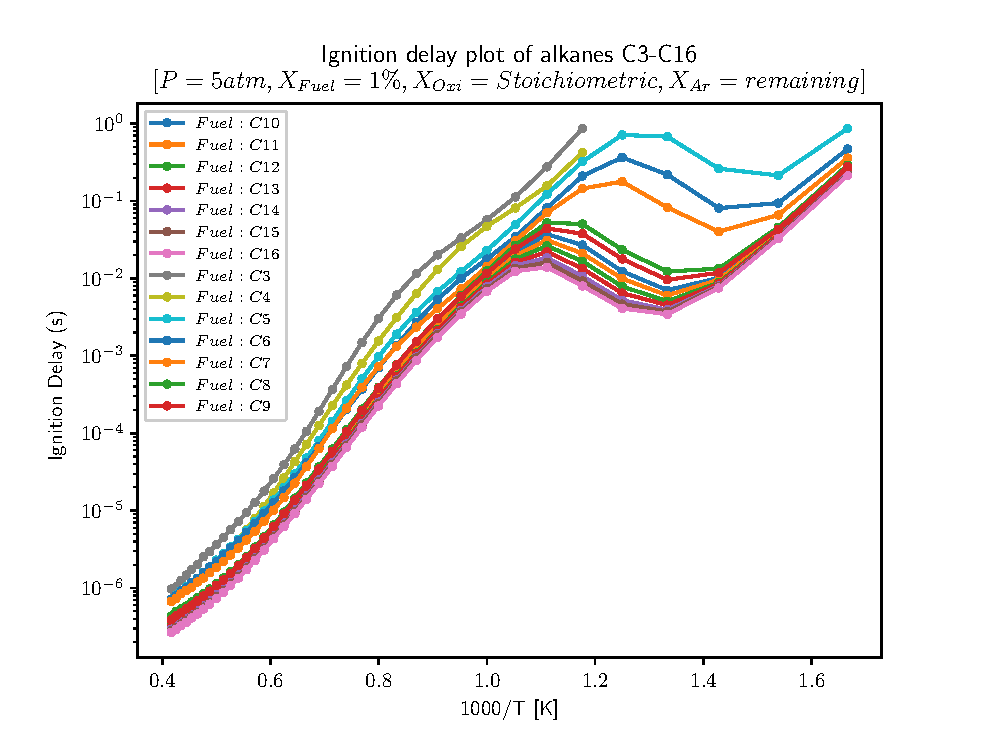
\includegraphics[scale=0.52]{combined_full_5.eps}}
			\hspace{0.25cm}
			\subfigure[Ignition delay result of C3-C16 alkanes at 10atm  ]{\label{fig:10atmfull}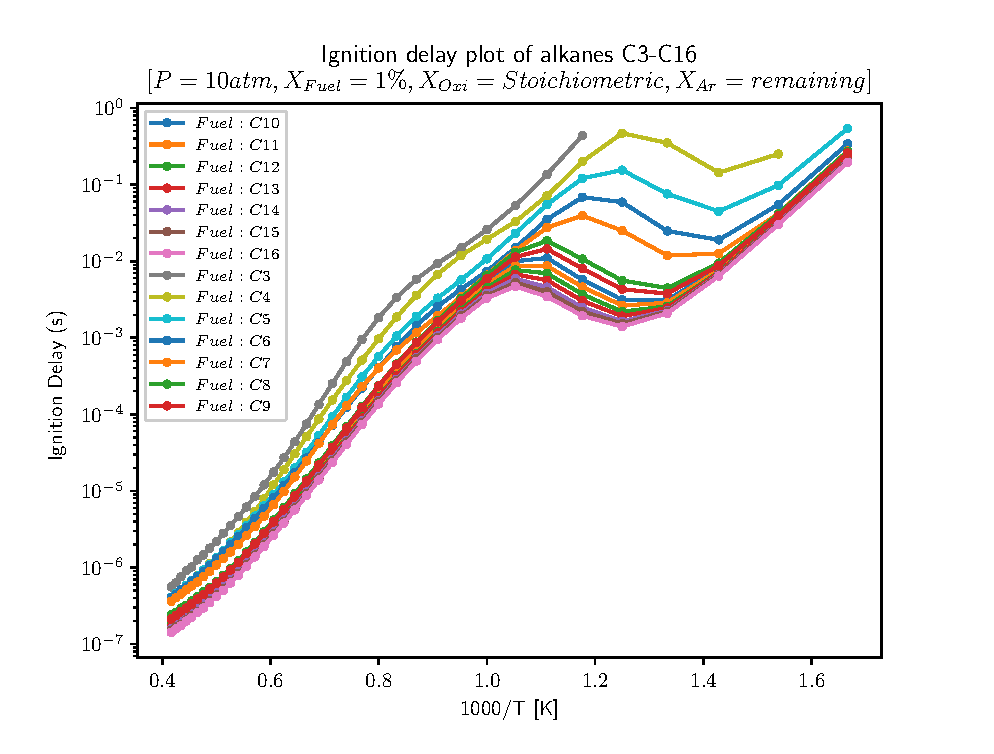
\includegraphics[scale=0.52]{combined_full_10.eps}}
			\caption{Ignition delay result of C3 - C16 alkanes at P= 5atm and 10atm, $X_{Fuel}=1\%$, $X_{Oxygen}= $According to stochiometry, $X_{Ar}= Remaining$,T= 600 to 2400 K.}
		}
		\end{figure}
		Obtained $\frac{E_a}{R}$ values for different fuels are shown in figure-\ref{fig:Ea_5full} and \ref{fig:Ea_10full}. All blue points shows $\frac{E_a}{R}$ value obtained by performing regression over simulation result. Plotting the  $\frac{E_a}{R}$ against number of secondary carbon-hydrogen bonds-$C_{SH}$ gives hidden information regarding relationship between two parameters. Detail of $C_{SH}$ bonds are illustrated in fig-\ref{fig:fuelbondtikz} by taking example of pentane. 
		
		 In figure-\ref{fig:Ea_5half} and \ref{fig:Ea_10half}, points shows $\frac{E_a}{R}$ values obtained by regression considering data within temperature range of 1800 to 1250 K. Each data point of $\frac{E_a}{R}$ is associated with each fuel. Same way, points in figure-\ref{fig:Ea_5full} and \ref{fig:Ea_10full} were obtained by performing regression considering all data from T= 600 to 2400 K.
		 By looking at trend of data points, intuitively it looks obvious that $\frac{E_a}{R}$ data follows nearly inversely proportional relationship with $C_{SH}$.
		   

	\begin{figure}[H]
			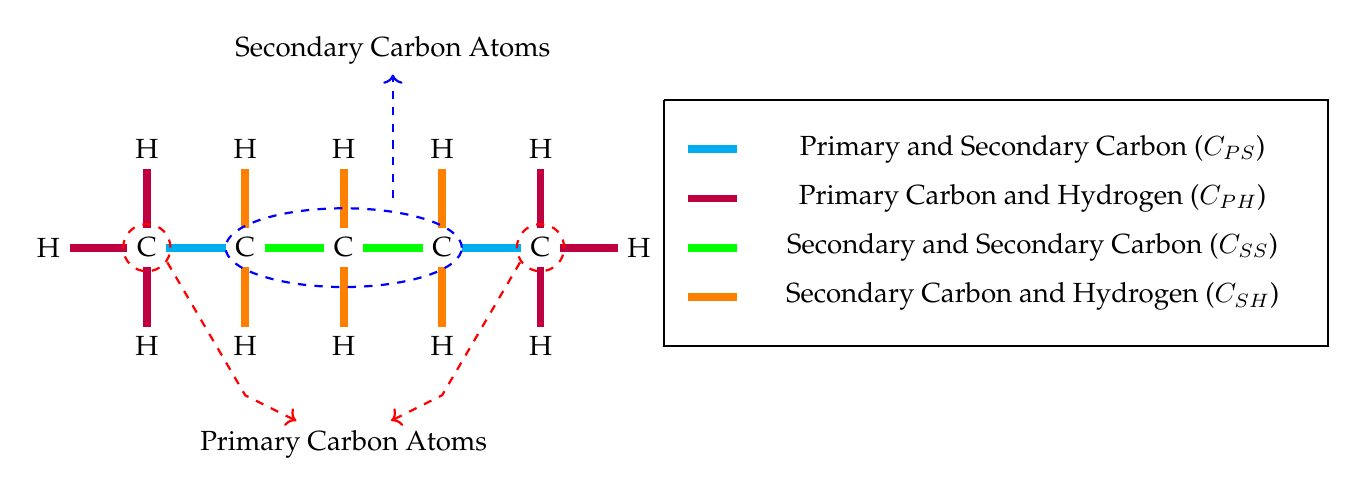
\begin{tikzpicture}[x=1.25cm,y=1.25cm]
					%Nodes Defined
					\node at (0,0) (nodeHstart) {H};
					\node at (1,0) (nodeC1) {C};
					\node at (1,1) (nodeC1H1) {H};
					\node at (1,-1) (nodeC1H-1) {H};
					\node at (2,0) (nodeC2) {C};
					\node at (2,1) (nodeC2H2) {H};
					\node at (2,-1) (nodeC2H-2) {H};
					\node at (3,0) (nodeC3) {C};
					\node at (3,1) (nodeC3H3) {H};
					\node at (3,-1) (nodeC3H-3) {H};
					\node at (4,0) (nodeC4) {C};
					\node at (4,1) (nodeC4H4) {H};
					\node at (4,-1) (nodeC4H-4) {H};
					\node at (5,0) (nodeC5) {C};
					\node at (5,1) (nodeC5H5) {H};
					\node at (5,-1) (nodeC5H-5) {H};
					\node at (6,0) (nodeHend) {H};
					
					%connecting nodes by drawing
					\draw[line width=1mm,purple] (nodeHstart) -- (nodeC1);
					\draw[line width=1mm,purple] (nodeC1) -- (nodeC1H1);
					\draw[line width=1mm,purple] (nodeC1) -- (nodeC1H-1);
					\draw[line width=1mm,cyan] (nodeC1) -- (nodeC2);
					\draw[line width=1mm,orange] (nodeC2) -- (nodeC2H2);
					\draw[line width=1mm,orange] (nodeC2) -- (nodeC2H-2);
					\draw[line width=1mm,green] (nodeC2) -- (nodeC3);
					\draw[line width=1mm,orange] (nodeC3) -- (nodeC3H3);
					\draw[line width=1mm,orange] (nodeC3) -- (nodeC3H-3);
					\draw[line width=1mm,green] (nodeC3) -- (nodeC4);
					\draw[line width=1mm,orange] (nodeC4) -- (nodeC4H4);
					\draw[line width=1mm,orange] (nodeC4) -- (nodeC4H-4);
					\draw[line width=1mm,cyan] (nodeC4) -- (nodeC5);
					\draw[line width=1mm,purple] (nodeC5) -- (nodeC5H5);
					\draw[line width=1mm,purple] (nodeC5) -- (nodeC5H-5);
					\draw[line width=1mm,purple] (nodeC5) -- (nodeHend);
					
					%Circle
					\draw[red,thick,dashed] (1,0) circle (0.3cm);
					\draw[red,thick,dashed] (5,0) circle (0.3cm);
					\draw[blue,thick,dashed] (3,0) ellipse (1.5cm and 0.5cm);
					
					%circle node and arrow node
					\node at (1.15,-0.05) (StartCir){} ;
					\node at (3,-2) (ArrowTail){Primary Carbon Atoms};
					\node at (4.85,-0.05) (EndCir){};
					%drawing
					
					\draw[red,thick,dashed,->] (StartCir) -- (2,-1.5) -- (ArrowTail);
					\draw[red,thick,dashed,->] (EndCir) -- (4,-1.5) -- (ArrowTail);
					
					%circle node and arrow node Secondary carbon
					\node at (3.5,2) (endSec) {Secondary Carbon Atoms};
					\draw[blue,thick,dashed,->] (3.5,0.5) -- (endSec) ;
					
					%representing colours 
					\draw[line width=0.25mm] (6.25,1.5) --(13,1.5) -- (13,-1) -- (6.25,-1) -- (6.25,1.5) ;
					\draw[line width=1mm,cyan](6.5,1)--(7,1) ;
					\node at (10,1) (PS) {Primary and Secondary Carbon  ($C_{PS}$)};
					
					\draw[line width=1mm,purple](6.5,0.5)--(7,0.5) ;
					\node at (10,0.5) (PS) {Primary Carbon and Hydrogen ($C_{PH}$)};
					
					\draw[line width=1mm,green](6.5,0)--(7,0) ;
					\node at (10,0) (PS) {Secondary and Secondary Carbon ($C_{SS}$)};
					
					\draw[line width=1mm,orange](6.5,-0.5)--(7,-0.5) ;
					\node at (10,-0.5) (PS) {Secondary Carbon and Hydrogen ($C_{SH}$)};
					\end{tikzpicture}						
				\caption{Different type of bonds in straight alkane (Pentane)}
				\label{fig:fuelbondtikz}
				\end{figure}
		
		To verify the relationship between $\frac{E_a}{R}$ and $C_{SH}$- (Number of secondary carbon-hydrogen bonds) used hypothesis is mentioned below:
		
		\begin{equation}\label{eq:Ea_regre}
		\begin{aligned}
		\frac{E_a}{R} &\propto \frac{1}{C_{SH}}\\
		\frac{E_a}{R} &\propto \beta_0 + \beta_1 \cdot \frac{1}{C_{SH}} \\
		\frac{E_a}{R} &\propto \beta_0 + \beta_1 \cdot {C_{SH}}^{-1}
		\end{aligned}
		\end{equation}
		
		By inverting $C_{SH}$ data and performing simple linear regression. Obtained regression coefficient and $R^2$ valued are mentioned in respective plots. All the values in fig-\ref{fig:Ea_5half}, \ref{fig:Ea_5full}, \ref{fig:Ea_10half}, \ref{fig:Ea_10full} shows promising results in favor of hypothesis with $R^2 > $0.84 for different cases.
		
		To maintain dimensionality, temperature term is used as proportionality constant. 
		
		\begin{equation}\label{eq:formulation_Ea}
		\begin{aligned}
		\frac{E_a}{R} &= T_0 \cdot \beta_0 + \beta_1 \cdot \frac{T_0}{C_{SH}}
		\end{aligned}
		\end{equation}
		
			
	
		\begin{figure}[H]\label{fig:Ea_Full}
			{
				\subfigure[$E_a/R$ vs Number of $C_{SH}$ at 5atm]{\label{fig:Ea_5half}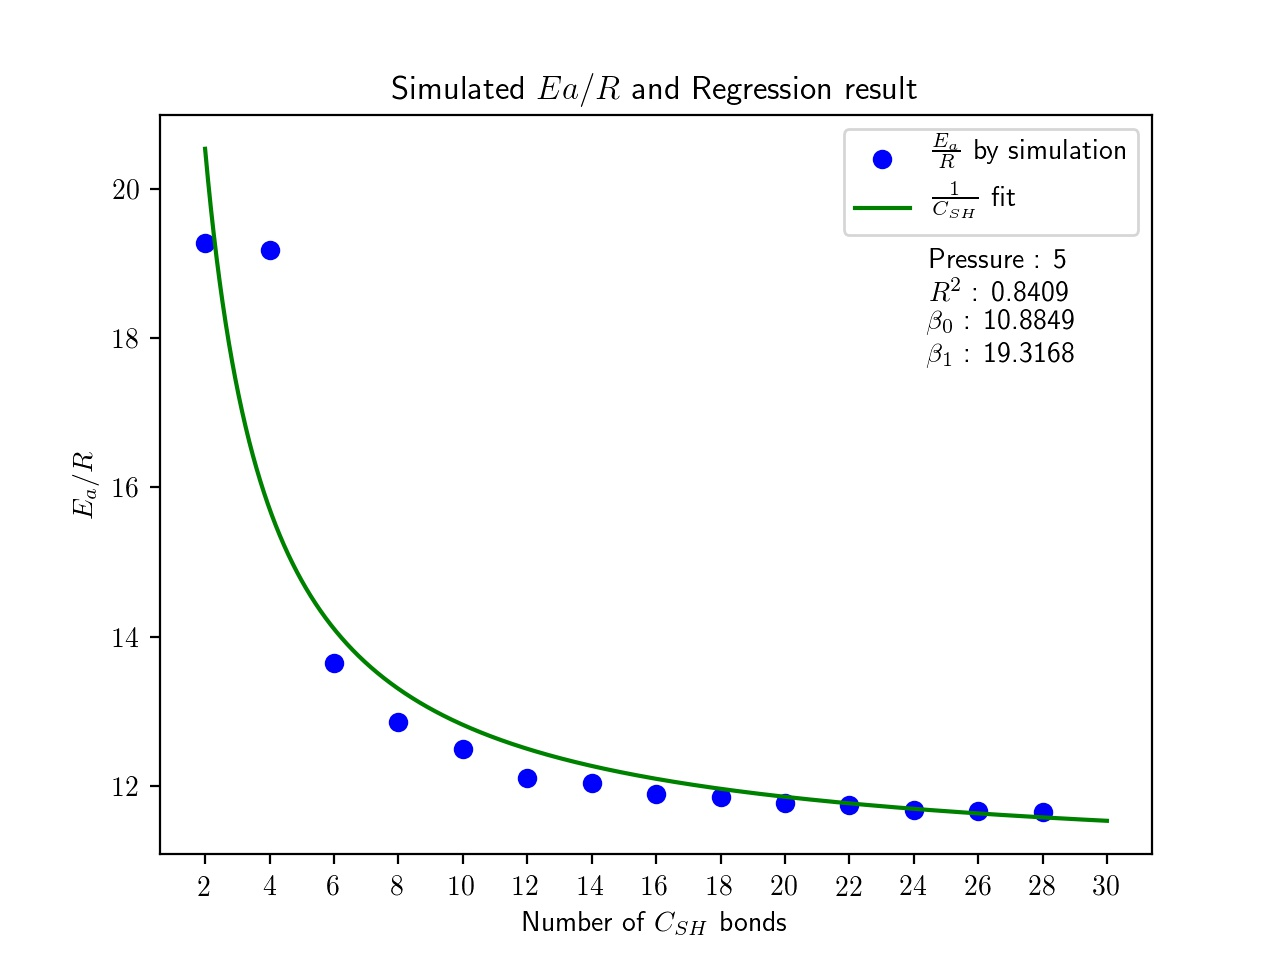
\includegraphics[scale=0.5]{comparision_Simulation_5_Half.jpg}}
				\hspace{0.25cm}
				\subfigure[$E_a/R$ vs Number of $C_{SH}$ at 10atm ]{\label{fig:Ea_10half}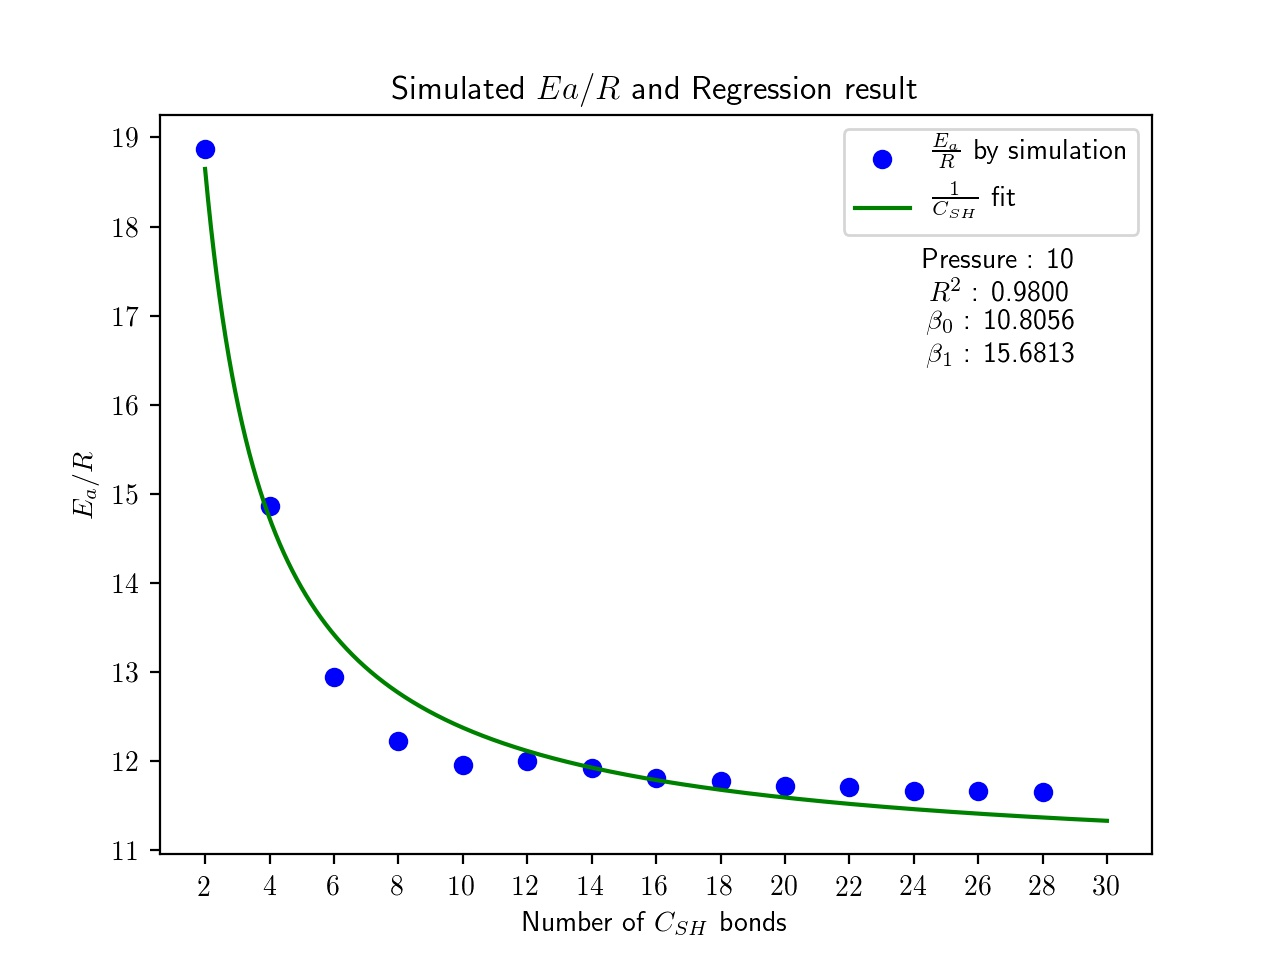
\includegraphics[scale=0.5]{comparision_Simulation_10_Half.jpg}}
				\caption{$E_a/R$ (using data ranges from 600 to 2400K) vs number $C_{SH}$ bonds and also its regression fit}
			}
		\end{figure}
		
		\begin{figure}[H]\label{fig:Ea_Half}
			{
				\subfigure[$E_a/R$ vs Number of $C_{SH}$ at 5atm]{\label{fig:Ea_5full}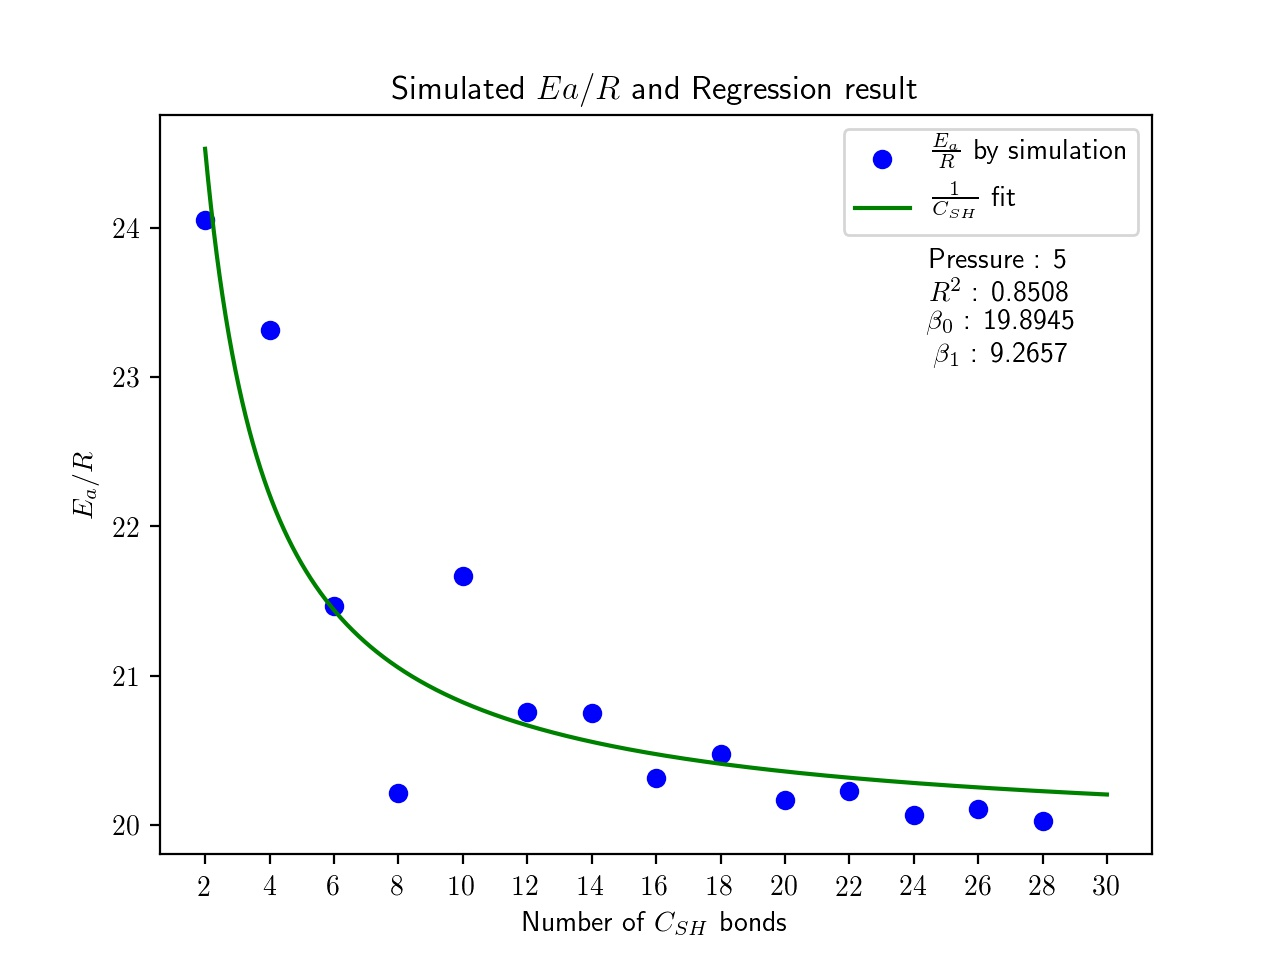
\includegraphics[scale=0.5]{comparision_Simulation_5_Full.jpg}}
				\hspace{0.25cm}
				\subfigure[$E_a/R$ vs Number of $C_{SH}$ at 10atm]{\label{fig:Ea_10full}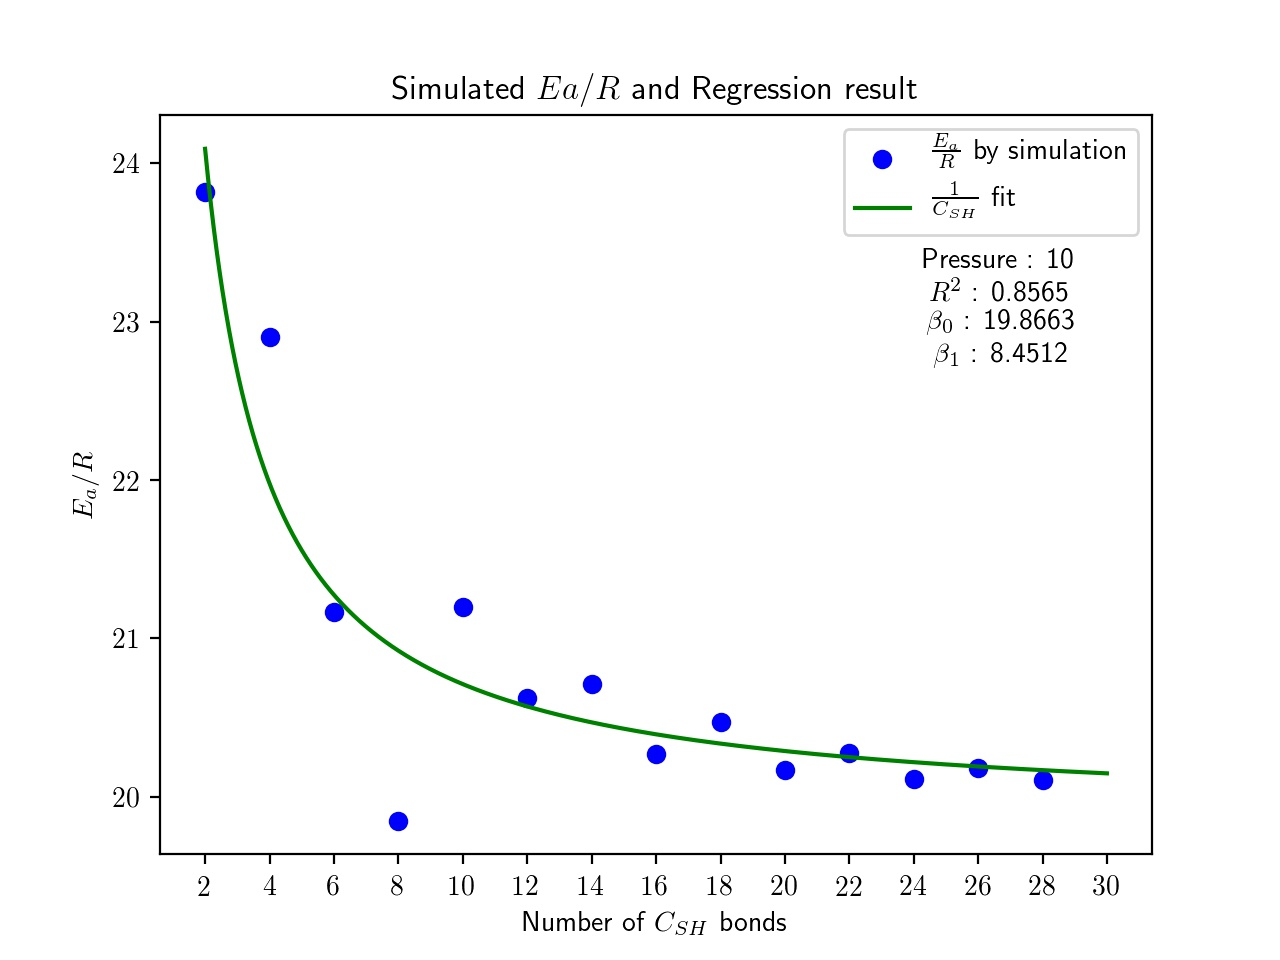
\includegraphics[scale=0.5]{comparision_Simulation_10_Full.jpg}}
				\caption{$E_a/R$ (using data ranges from 1250 to 1800K) vs number $C_{SH}$ bonds and also its regression fit}
			}
		\end{figure}
		
			From equation- (\ref{eq:formula__comparision_full}) and (\ref{eq:formulation_Ea}) the obtain term can be written as,
			
			\begin{equation}\label{eq:formularion_comparision_Ea}
			\begin{aligned}		
			\bigg\{\underbrace{\frac{\text{Constant Energy Term}}{R} + \frac{\text{ Fuel Bond Energy Term}}{R} }_{term-A}\bigg\} &\sim \underbrace{(\alpha_0 \cdot T_0 + \alpha_1 \cdot T_0 )}_{term-B} &\sim \underbrace{(T_0 \cdot \beta_0 + \beta_1 \cdot \frac{T_0}{C_{SH}}}_{term-C}\bigg\}\\
			\end{aligned}
			\end{equation}
			
			Replacing term-A of formulation-\ref{eq:formulation1} with term-C mentioned above, gives final formulation for ignition delay with replacement of activation energy with bond details - \ref{eq:final_formulation}.
			
			\begin{equation}\label{eq:final_formulation}
			\begin{aligned}		
			\tau &\propto  \phi^\alpha \cdot P^\beta  \cdot X_{O_2}^\gamma   \cdot \exp \bigg( \frac{1}{T} \cdot \bigg\{ T_0 \cdot \beta_0 + \beta_1 \cdot \frac{T_0}{C_{SH}}\bigg\} \bigg)	
			\end{aligned}
			\end{equation}
			
		
	 This formulation gives clear indication regarding, ignition delay dependency on the fuel bonds. To make quantities independent of unit, some terms in the formulation is normalized with unit quantities. Considering all the possible affecting parameters in above formulation-\ref{eq:final_formulation}, the functional form it can be expressed as:	
		  \begin{equation}\label{eq:functional}
		  \begin{aligned}
\tau = f(T,P,\phi,X_{Fuel},X_{O_2},X_{Dilutant},C_{SH})
		  \end{aligned}
		  \end{equation}
		 \hspace{0.25cm}But it is known that ,
		 
		 \begin{equation}
		 \begin{aligned}
			X_{Fuel}+X_{O_2}+X_{Dilut6ant} = 1
			 \hspace{0.5cm} \& \hspace{0.5cm}
		 \phi = \frac{\bigg(\frac{X_{fuel}}{X_{O_2}}\bigg)_{act}}{\bigg(\frac{X_{fuel}}{X_{O_2}}\bigg)_{stochio}}
	 	\end{aligned}
	 	\end{equation}
	 	As Fuel composition is already known, from stoichiometry equation,  $\bigg(\frac{X_{fuel}}{X_{O_2}}\bigg)_{stochio}$ is attainable. It is possible to obtain $\phi$ from $X_{fuel}$ and $X_{O_2}$, which is also true for $X_{Diluant}$. 
	 	
	 	 Removing redundant function formulation can be re-written  as,
	 	\begin{equation}\label{eq:func}
	 	\begin{aligned}
	 	\tau = f(T,P,X_{Fuel},X_{O_2},C_{SH})
	 	\end{aligned} 
	 	\end{equation}
	 	
	 		\begin{equation}
	 		\begin{aligned}
	 		\tau &\propto \bigg(\frac{P}{P_0}\bigg)^b  \cdot X_{Fuel}^c    \cdot X_{O_2}^d    \cdot exp\Bigg( \beta_0 \cdot \frac{T_0}{T} + \beta_1 \cdot \frac{T_0}{T \cdot C_{SH}} \Bigg) \\
	 		&= C' \cdot \bigg(\frac{P}{P_0}\bigg)^b  \cdot X_{Fuel}^c    \cdot X_{O_2}^d    \cdot exp\Bigg( \beta_0 \cdot \frac{T_0}{T} + \beta_1 \cdot \frac{T_0}{T \cdot C_{SH}} \Bigg) \\\\
	 		\end{aligned}
	 		\end{equation}
	 		
	 	Formulation can simplified by taking natural log on both side,
		\begin{equation}\label{eq:hypo_ignition}
			\begin{aligned}
			ln(\tau) &= ln(C') + b \cdot ln(\frac{P}{P_0})+ c \cdot ln(X_{Fuel})+    d \cdot ln(X_{O_2}) + \beta_0 \cdot \frac{T_0}{T} + \beta_1 \cdot \frac{T_0}{T \cdot C_{SH}} \\
			ln(\tau) &= C + b \cdot ln(\frac{P}{P_0})+ c \cdot ln(X_{Fuel})+    d \cdot ln(X_{O_2}) + \beta_0 \cdot \frac{T_0}{T} + \beta_1 \cdot \frac{T_0}{T \cdot C_{SH}}
			\end{aligned}
		\end{equation}
		
		
		
		where, C, b, c, d, $\beta_0,$ $\beta_1$ are coefficients, which is attainable from ignition delay data using multiple regression. It was assumed that ignition delay correlation depends on all the parameters which can be refined using hypothesis testing. To obtain models, multiple regression was used with error based clustering, which explained in further discussion. The fundamental step of whole process is to collect the data and make ot processable, which is discussed in next section.
		
		
				
				\newpage	
			References:
					%%
					%% Following citation commands can be used in the body text:
					%% Usage of \cite is as follows:
					
					%%   \cite{key}          ==>>  [#]
					%%   \cite[chap. 2]{key} ==>>  [#, chap. 2]
					%%   \citet{key}         ==>>  Author [#]
					
					%% References with bibTeX database:
					
					\bibliographystyle{ieeetr}
					\bibliography{biblio.bib}
					
					%% Authors are advised to submit their bibtex database files. They are
					%% requested to list a bibtex style file in the manuscript if they do
					%% not want to use model1-num-names.bst.
					
					%% References without bibTeX database:
					
					% \begin{thebibliography}{00}
					
					%% \bibitem must have the following form:
					%%   \bibitem{key}...
					%%
					
					% \bibitem{}
					
					% \end{thebibliography}
					
					
				\end{document}
				
				%%
				%% End of file `elsarticle-template-1-num.tex'.